\section{Evaluation}
\label{sec:eval}

We evaluate Themis through benchmarks of several different MapReduce jobs on
both synthetic and real-world data sets.  A summary of
our results are as follows:

\begin{itemize}
  \item Themis is highly performant on a wide variety of MapReduce jobs, and
    outperforms Hadoop by 3x - 16x on a variety of common jobs.
  \item Themis can achieve nearly the sequential speed of the
  disks for I/O-bound jobs, which is approximately the same rate as TritonSort's
  record-setting performance.
  \item Themis's memory subsystem is flexible, and is able to handle
  large amounts of data skew while ensuring efficient operation.
\end{itemize}

\subsection{Workloads and Evaluation Overview}
\label{sec:methodology}

\begin{table*}
  \centering
  \caption{\label{table:description} A description and table of abbreviations
    for the MapReduce jobs evaluated in this section. Data sizes take into
    account 8 bytes of metadata per record for key and value sizes.}
  \resizebox{\columnwidth}{!}{
  \begin{tabular}{|c|p{3.2in}|c|c|c|}
    \hline
    & & \multicolumn{3}{|c|}{\textbf{Data Size}} \\ \cline{3-5}
    \textbf{Job Name}      & \centering \textbf{Description} & Input & Intermediate & Output \\
    \hline
    \hline
    Sort-100G     & Uniformly-random sort, 100GB per node & 2.16TB & 2.16TB & 2.16TB \\
    Sort-500G     & Uniformly-random sort, 500GB per node & 10.8TB & 10.8TB & 10.8TB \\
    Sort-1T       & Uniformly-random sort, 1TB per node & 21.6TB & 21.6TB & 21.6TB\\
    Sort-1.75T    & Uniformly-random sort, 1.75TB per node & 37.8TB & 37.8TB & 37.8TB\\
    \hline
    Pareto-1M     & Sort with Pareto-distributed key/value sizes, $\alpha=1.5$, $x_0=100$ (1MB max key/value size) & 10TB & 10TB & 10TB\\
    Pareto-100M   & Sort with Pareto-distributed key/value sizes, $\alpha=1.5$, $x_0=100$ (100MB max key/value size) & 10TB & 10TB & 10TB\\
    Pareto-500M   & Sort with Pareto-distributed key/value sizes, $\alpha=1.5$, $x_0=100$ (500MB max key/value size) & 10TB & 10TB & 10TB\\
    \hline
    CloudBurst    & CloudBurst (two nodes, performing alignment on
    \texttt{lakewash\_combined\_v2.genes.nucleotide}) & 971.3MB & 68.98GB & 517.9MB\\
    \hline
    PageRank-U    & PageRank (synthetic uniform graph, 25M vertices, ~50K
    random edges per vertex) & 1TB & 4TB & 1TB \\
    PageRank-PL   & PageRank (synthetic graph with power-law vertex in-degree,
    250M vertices)  & 934.7GB & 3.715TB & 934.7GB\\
    PageRank-WEX  & PageRank on WEX page graph & 1.585GB & 5.824GB & 2.349GB\\
    \hline
    WordCount & Count words in text of WEX & 8.22GB & 27.74GB & 812MB \\
    \hline
    n-Gram & Count 5-grams in text of WEX & 8.22GB & 68.63GB & 49.72GB \\
    \hline
    Click-Sessions & Session extraction from 2TB of synthetic click logs & 2TB
    & 2TB & 8.948GB \\
    \hline
  \end{tabular}
}
\end{table*}

We evaluate Themis on the cluster described in
Section~\ref{sec:hardware_architecture}. Each XFS partition is configured with
a single allocation group to prevent file fragmentation across allocation
groups, and is mounted with the \texttt{noatime} flag set. For this evaluation,
all servers were running Linux 2.6.32. Our implementation of Themis is written
in C++ and is compiled with g++ 4.6.2.

To evaluate Themis at scale, we often have to rely on large
synthetically-generated data sets, due to the logistics of obtaining and
storing freely-available, large data sets.  All synthetic data sets are
evaluated on 20 cluster nodes. Non-synthetic data sets are small enough to
be evaluated on a single node.

All input and output data is stored on local disks without using any
distributed filesystem and without replication. We explore Themis's interaction
with distributed storage in Chapter~\ref{chapter:fault_tolerance}.

We evaluate Themis's performance on several different MapReduce jobs. A
summary of these jobs is given in Table~\ref{table:description}, and each job
is described in more detail below.

\subsubsection{Sort}

Large-scale sorting is a useful measurement of the
performance of MapReduce and of data processing systems in general.  During a
sort job, all cluster nodes are reading from disks, writing to disks, and doing
an all-to-all network transfer simultaneously.  Sorting also measures the
performance of MapReduce independent of the computational complexity of the
\map and \reduce functions themselves, since both \map and \reduce functions
are effectively no-ops. We study the effects of both increased data density and
skew on the system using sort due to the convenience with which input data that
meets desired specifications can be generated.  We generate skewed data with a
Pareto distribution.  The record size in generated datasets is limited by a
fixed maximum, which is a parameter given to the job.

\subsubsection{WordCount}

Word count is a canonical MapReduce job. Given a
collection of words, word count's \map function emits \kvpair{word}{1} records
for each word.  Word count's \reduce function sums the occurrences of each word
and emits a single \kvpair{word}{N} record, where N is the number of times
the word occurred in the original collection.

We evaluate WordCount on the 2012-05-05 version of the Freebase Wikipedia
Extraction (WEX)~\cite{wex}, a processed dump of the English version of
Wikipedia. The complete WEX dump is approximately 62GB uncompressed, and
contains both XML and text versions of each page. We run word count on the text
portion of the WEX data set, which is approximately 8.2GB uncompressed.

\subsubsection{n-Gram Count}

 An extension of word count, n-gram count counts the
number of times each group of $n$ words appears in a text corpus. For
example, given ``The quick brown fox jumped over the lazy dog'', 3-gram count
would count the number of occurrences of ``The quick brown'', ``quick brown
fox'', ``brown fox jumped'', etc. We also evaluate n-gram count on the text
portion of the WEX data set.

\subsubsection{PageRank}

PageRank is a graph algorithm that is widely used by
search engines to rank web pages.  Each node in the graph is given an initial
rank. Rank propagates through the graph by each vertex contributing a fraction
of its rank evenly to each of its neighbors.

PageRank's \map function is given a record for each vertex in the graph whose
key is the vertex's ID and whose value is a concatenation of the vertex's
adjacency list and its initial rank. The \map function emits \kvpair{adjacent
  vertex ID}{rank contribution} pairs for each adjacent vertex ID, and also
re-emits the adjacency list so that the graph can be reconstructed. PageRank's
\reduce function adds the rank contributions for each vertex to compute that
vertex's rank, and emits the vertex's existing adjacency list and new rank.

We evaluate PageRank with three different kinds of graphs. The first
(PageRank-U) is a 25M vertex synthetically-generated graph where each vertex
has an edge to every other vertex with a small, constant probability. Each
vertex has an expected degree of 5,000. The second (PageRank-PL) is a 250M
vertex synthetically-generated graph where vertex in-degree follows a power law
distribution with values between 100 and 10,000. This simulates a more realistic
page graph where a relatively small number of pages are linked to
frequently. The third (PageRank-WEX) is a graph derived from page links in the
XML portion of the WEX data set; it is approximately 1.5GB uncompressed and has
~5.3M vertices.

\subsubsection{CloudBurst}

CloudBurst~\cite{cloudburst-bio} is a MapReduce
implementation of the RMAP~\cite{rmap} algorithm for short-read gene alignment,
which aligns a large collection of small ``query'' DNA sequences called
\emph{reads} with a known ``reference'' genome. CloudBurst performs this
alignment using a standard technique called \emph{seed-and-extend}. Both query
and reference sequences are passed to the \map function and emitted as a series
of fixed-size \emph{seeds}. The \map function emits seeds as sequence of
\kvpair{seed}{seed metadata} pairs, where the seed metadata contains
information such as the seed's location in its parent sequence, whether that
parent sequence was a query or a reference, and the characters in the sequence
immediately before and after the seed.

CloudBurst's \reduce function examines pairs of query and reference strings with
the same seed. For each pair, it computes a similarity score of the DNA
characters on either side of the seed using the Landau-Vishkin algorithm for
approximate string matching. The \reduce function emits all query/reference
pairs with a similarity score above a configured threshold.

We evaluate CloudBurst on the lakewash\_combined\_v2 data set from University
of Washington~\cite{cloudburst_uw_data}, which we pre-process using a slightly
modified version of the CloudBurst input loader used in Hadoop.

\subsubsection{Click Log Analysis}

Another popular MapReduce job is analysis of click logs. Abstractly, click logs
can be viewed as a collection of \kvpair{user ID}{timestamp|URL} pairs (where
the \texttt{|} symbol denotes the concatenation of logical fields as part of
the value) indicating which page a user loaded at which time.  We chose to
evaluate one particular type of log analysis task, \emph{session tracking}. In
this task, we seek to identify disjoint ranges of timestamps at least some
number of seconds apart. For each such range of timestamps, we output
\kvpair{user ID}{start timestamp|end timestamp|start URL|end URL} pairs.

The \map function is a pass-through; it simply groups records by user ID. The
\reduce function does a linear scan through records for a given user ID and
reconstructs sessions. For efficiency, it assumes that these records are sorted
in ascending order by timestamp. We describe the implications of this
assumption in the next section.

\subsection{Job Implementation Details}

In this section, we briefly describe some of the implementation details
necessary for running our collection of example jobs at maximum efficiency.

\subsubsection{Combiners}

A common technique for improving the performance of
MapReduce jobs is employing a \emph{combiner}. For example, word count can emit
a single \kvpair{word}{$k$} pair instead of $k$ \kvpair{word}{1}
pairs. Themis supports the use of combiner functions. We opted to implement
combiners within the \mapper stage on a job-by-job basis rather than adding an
additional stage.  Despite what conventional wisdom would suggest, we found
that combiners actually decreased our performance in many cases
because the computational overhead of manipulating large data structures was
enough to make the \mapper compute-bound. The large size of these data
structures is partially due to our decision to run the combiner over an entire
job's intermediate data rather than a small portion thereof to
maximize its effectiveness.

In some cases, however, a small data structure that takes advantage of the
semantics of the data provides a significant performance increase. For example,
our word count MapReduce job uses a combiner that maintains a counter for the
top 25 words in the English language.  The combiner updates the appropriate
counter whenever it encounters one of these words rather than creating an
intermediate record for it.  At the end of phase one, intermediate records are
created for each of these popular words based on the counter values.

\subsubsection{Improving Performance for Small Records}

The \map functions in our first implementations of word count and n-gram count
emitted \kvpair{<word/n-gram}{1} pairs. Our implementations of these \map
functions emit \kvpair{hash(word)}{1|word} pairs instead because the resulting
intermediate partitions are easier to sort quickly because the keys are all
small and the same size.

\subsubsection{Secondary Keys}

A na\"{\i}ve implementation of the session extraction job sorts records for a
given user ID by timestamp in the \reduce function. We avoid performing two
sorts by allowing the \Sorter stage to use the first few bytes of the value,
called a \emph{secondary key}, to break ties when sorting. For example, in the
session extraction job the secondary key is the record's timestamp.

\subsection{Performance}

We evaluate the performance of Themis in two ways. First, we compare
performance of the benchmark applications to the cluster's hardware
limits. Second, we compare the performance of Themis to that of Hadoop on two
benchmark applications.

\subsubsection{Performance Relative to Disk Speeds}

\begin{figure}
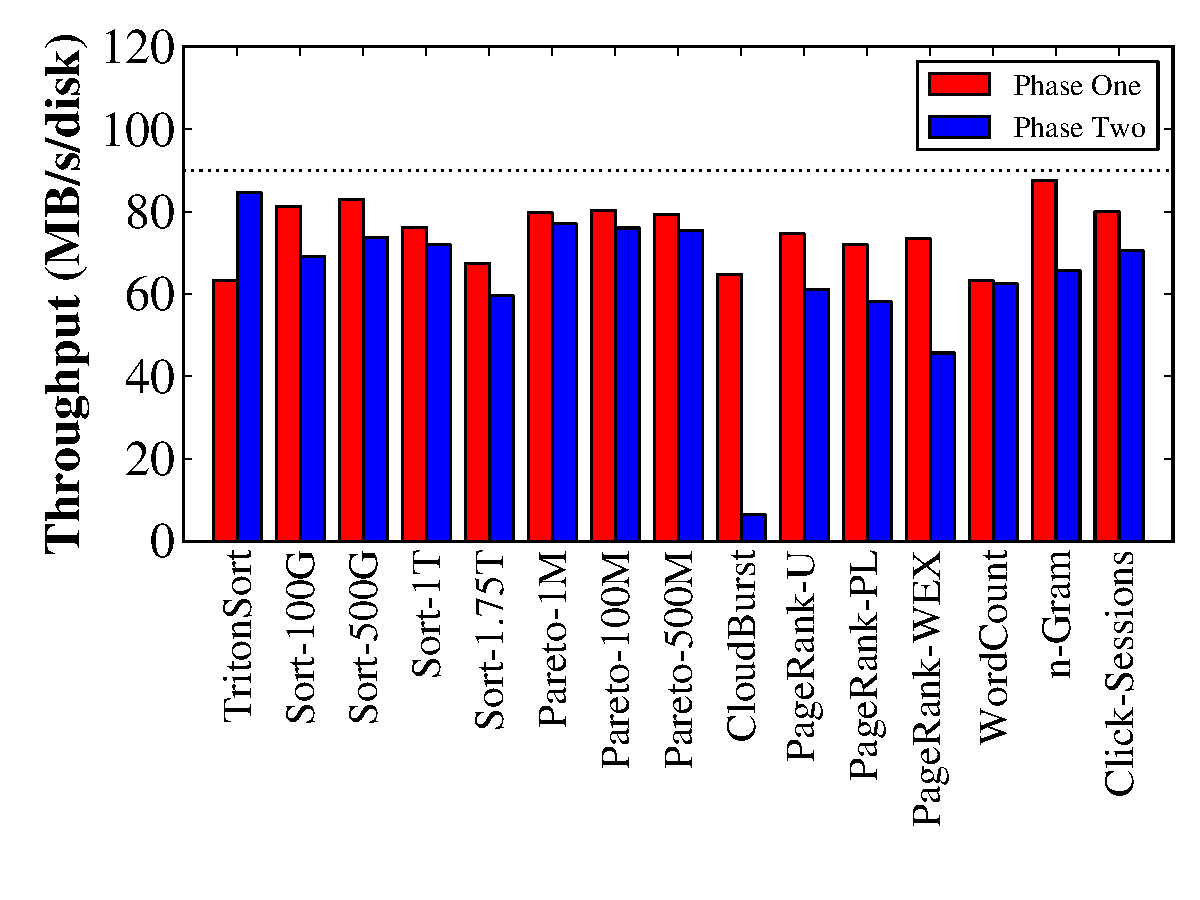
\includegraphics[width=\columnwidth]{themis/graphs/performance.pdf}
\caption{\label{fig:performance} Performance of evaluated MapReduce
  jobs. Maximum sequential disk throughput of approximately 90 MB/s is shown as
  a dotted line. Our TritonSort record from 2011 is shown on the left for
  comparison.}
\end{figure}

The performance of Themis on the benchmark MapReduce jobs is shown in
Figure~\ref{fig:performance}. Performance is measured in terms of
\emph{MB/s/disk} in order to provide a relative comparison to the hardware
limitations of the cluster. The 7200 RPM drives in the cluster are capable of
approximately 90 MB/s/disk of sequential write bandwidth, which is shown as a
dotted line in the figure. A job running at 90 MB/s/disk is processing data as
fast as it can be written to the disks.

Most of the benchmark applications run at near maximum speed in both
phases. CloudBurst's poor performance in phase two is due to the
computationally intensive nature of its \reduce function, which is unable to
process records fast enough to saturate the disks. More CPU cores are needed to
drive computationally intensive applications such as CloudBurst at maximum
speed in both phases. Notice however that CloudBurst is still able to take
advantage of our architecture in phase one.

We have included TritonSort's performance on the Indy 100TB sort benchmark for
reference. TritonSort's 2011 Indy variant runs a much simpler code base than
Themis. We highlight the fact that Themis's additional complexity and
flexibility does not impact its ability to perform well on a variety of
workloads. Our improved performance in phase one relative to TritonSort at
scale is due to a variety of internal improvements and optimizations made to
the codebase in the intervening period, as well as the improved memory
utilization provided by moving from buffer pools to dynamic memory
management. Performance degradation in phase two relative to TritonSort is
mainly due to additional CPU and memory pressure introduced by the \Reducer
stage.

\subsubsection{Comparison with Hadoop}

\begin{table}
  \centering
  \caption{\label{table:hadoop} Performance comparison of Hadoop and Themis.}
  \begin{tabular}{|c|c|c|c|}
    \hline
     & \multicolumn{2}{|c|}{\textbf{Running Time}} &
     \\
    \cline{2-3}
    \textbf{Application} & Hadoop & Themis & \textbf{Improvement}\\
    \hline
    Sort-500G & 28881s & 1789s & 16.14x \\
    CloudBurst & 2878s & 944s & 3.05x \\
    \hline
  \end{tabular}
\end{table}

We evaluate Hadoop version 1.0.3 on the Sort-500G and CloudBurst
applications. We started with a configuration based on the configuration used
by Yahoo! for their 2009 Hadoop sort record~\cite{terasort}. We optimized
Hadoop as best we could, but found it difficult to get it to run many large
parallel transfers without having our nodes blacklisted for running out of
memory.

The total running times for both Hadoop and Themis are given in
Table~\ref{table:hadoop}. I/O-bound jobs such as sort are able to take full
advantage of our architecture, which explains why Themis is more than a factor
of 16 faster. As explained above, CloudBurst is fundamentally compute-bound,
but the performance benefits of the 2-IO property allow the Themis
implementation of CloudBurst to outperform the Hadoop implementation by a
factor of 3.

\subsection{Memory Management}

In this section, we evaluate the performance of our different memory allocation
policies. We also show that our allocation system is robust in the face of
transient changes in individual stage throughputs.

\subsubsection{Memory Allocator Performance}

\begin{figure}
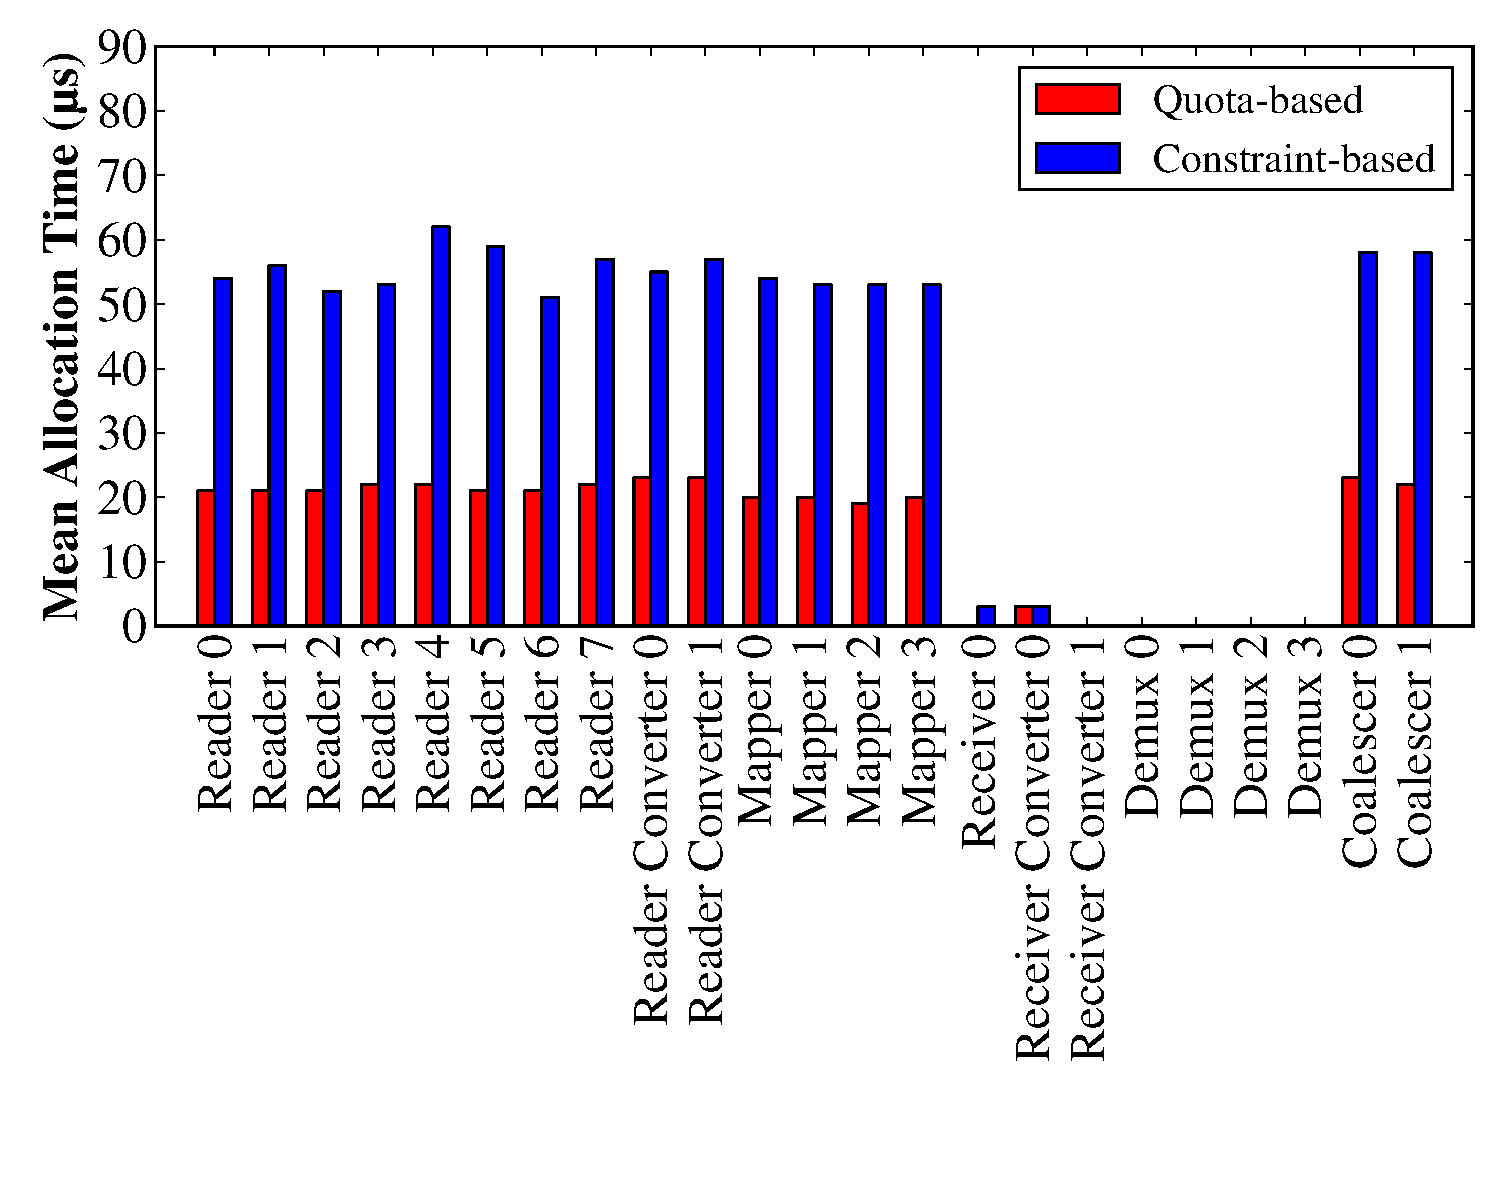
\includegraphics[width=\columnwidth]{themis/graphs/allocation_time_means.pdf}
\caption{\label{fig:allocation_time_means} Effects of allocation policy on mean
allocation times across workers.}
\end{figure}

\begin{table}
  \centering
  \caption{\label{table:allocator_end_to_end_performance} Performance of
    allocation policies.}
  \begin{tabular}{|c|c|}
    \hline
    \textbf{Allocation Policy} & \textbf{Phase One Throughput} \\
    \hline
    Constraint-Based & 84.90 MBps/disk \\
    Quota-Based & 83.11 MBps/disk \\
    \hline
  \end{tabular}
\end{table}

We examine both the individual allocation times of our different memory
allocation policies and their end-to-end performance.  We evaluate the
performance on phase one of a 200GB, 1-node sort
job. Table~\ref{table:allocator_end_to_end_performance} shows that phase one's
throughput is essentially unaffected by the choice of allocator policy in this
particular instance. These performance numbers can be explained by looking at
the mean allocation time for each worker in the
system. Figure~\ref{fig:allocation_time_means} shows that while the
constraint-based allocator is more than twice as slow as the quota-based
allocator, the absolute allocation times are both measured in tens of
microseconds, which is negligible compared to time taken to actually do useful
work.

However, the results above only hold in the case where the constraint-based
allocator does not deadlock. While we never experienced deadlock in phase two,
we found it was quite easy to construct situations in which phase one
deadlocked. For example, the exact same experiment conducted on a slightly
larger data set causes deadlock in phase one with the constraint-based
allocator.

The performance results in Figure~\ref{fig:performance} demonstrate the
constraint-based allocation policy performs well in phase two.  Because phase
two handles entire intermediate partitions in memory, its allocations are
orders of magnitude larger than those in phase one. This dramatically increases
the likelihood that a single memory request is larger than one of the phase's
quotas.

\subsubsection{Robustness of the Quota-Based Memory Allocation Policy}

\begin{figure}
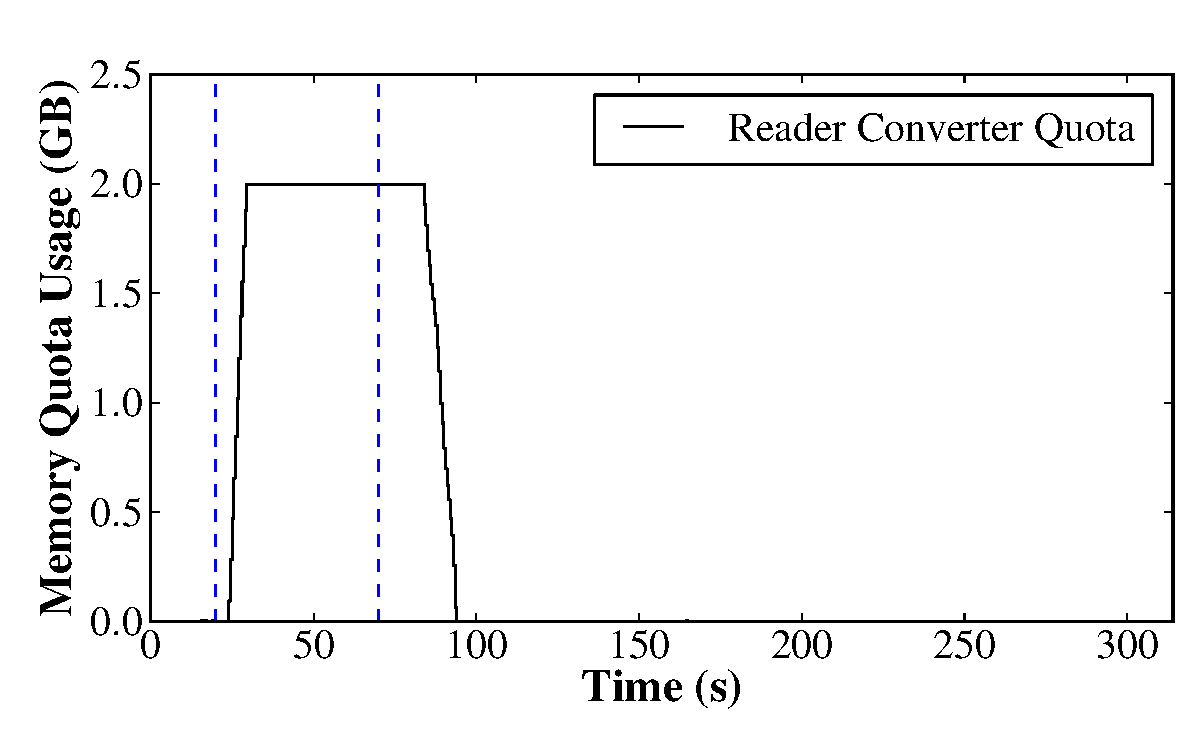
\includegraphics[width=\columnwidth]{themis/graphs/reader_converter_quota_slow_network.pdf}
\caption{\label{fig:reader_converter_quota_slow_network} Memory quota usage of
  the Reader Converter stage. The network was made artificially slow in the
  time period designated by the dashed lines.}
\end{figure}

We evaluate the robustness of the quota-based memory allocator by artificially
slowing down the network for a period of time. We observe the effect on the
total quota usage of a stage in the pipeline. Figure
\ref{fig:reader_converter_quota_slow_network} shows that the Reader Converter's
quota usage spikes up to its limit of 2GB in response to a slow network and
then returns back to a steady state of near 0. A slow network means that stages
upstream of the network are producing data faster than the network can transmit
data. This imbalance leads to data backing up in front of the
network. In the absence of the quota allocation policy, this data backlog grows
unbounded.

\subsection{Skew Mitigation}

\begin{figure}
  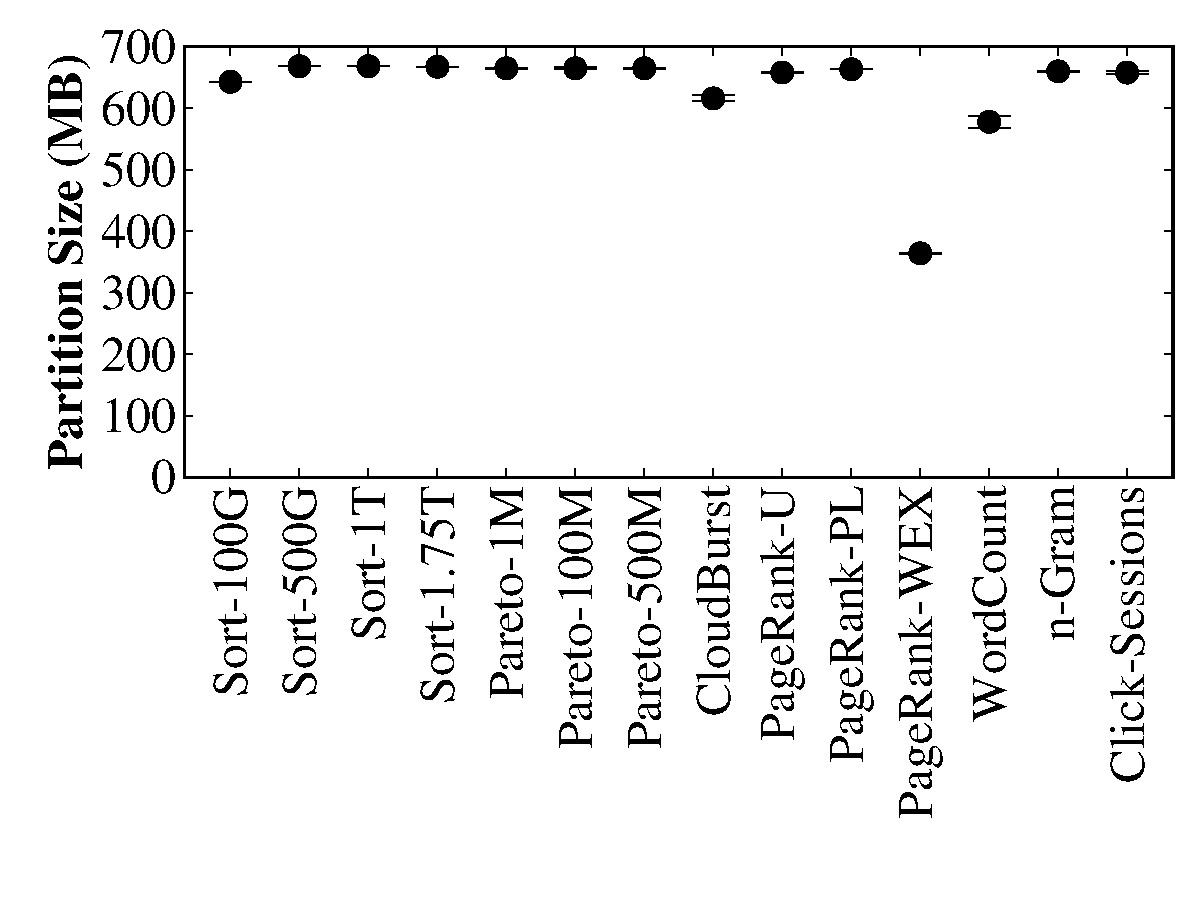
\includegraphics[width=\columnwidth]{themis/graphs/ld_sizes_plot.pdf}
  \caption{\label{fig:ld_sizes} Partition sizes for various Themis
    jobs. Error bars denoting the 95\% confidence intervals are hard to see
    due to even partitioning.}
\end{figure}

Next, we evaluate Themis's ability to handle skew by observing the sizes of
the intermediate data partitions created in phase one.
Figure~\ref{fig:ld_sizes} shows the partition sizes produced by Themis on the
evaluated applications. The error bars denoting the 95\% confidence intervals
are small, indicating that all partitions are nearly equal in size. This is
unsurprising for applications with uniform data, such as sort. However, Themis
also achieves even partitioning on very skewed data sets, such as
Pareto-distributed sort, PageRank, and WordCount. PageRank-WEX has fairly small
partitions relative to the other jobs because its intermediate data size is not
large enough for phase zero to create an integer number of partitions with the
desired size.

\subsection{Write Sizes}

\begin{figure}
  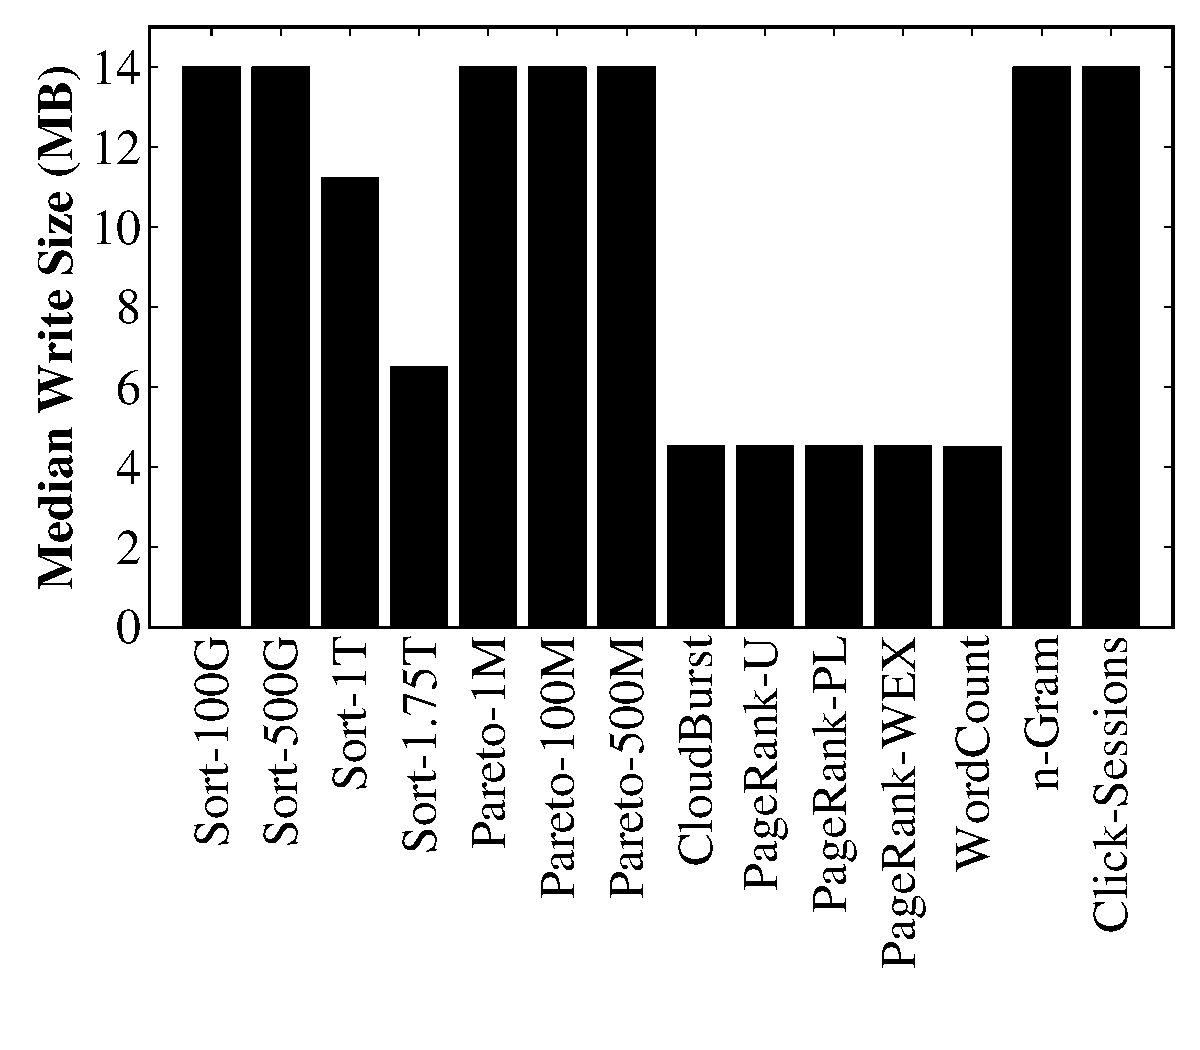
\includegraphics[width=\columnwidth]{themis/graphs/write_sizes_median_bars.pdf}
  \caption{\label{fig:write_sizes} Median write sizes for various Themis jobs.}
\end{figure}

One of primary goals of phase one is to do large writes to each partition to
avoid unnecessary disk seeks.  Figure~\ref{fig:write_sizes} shows the median
write sizes of the various jobs we evaluated.  For jobs like Sort and n-Gram
where the \map function is extremely simple and \mappers can map data as fast
as \readers can read it, data buffers up in the \Chainer stage and all writes
are large. As the amount of intermediate data per node grows, the size of a
chain that can be buffered for a given partition decreases, which fundamentally
limits the size of a write. For example, Sort-1.75T writes data to 2832
partitions, which means that its average chain length is not expected to be
longer than about 5 MB given a \receiver memory quota of 14GB; note, however,
that the mean write size is above this minimum value, indicating that the
\writer is able to take advantage of temporary burstiness in activity for
certain partitions.  If the stages before the \Writer stage cannot quite
saturate it (such as in WordCount, CloudBurst and PageRank), chains remain
fairly small. Here the minimum chain size of 4.5 MB ensures that writes are
still reasonably large. In the case of PageRank-WEX, the data size is
too small to cause the chains to ever become very large.
